\documentclass[tikz,border=5pt]{standalone}
\usepackage{pgfplots}
\pgfplotsset{compat=1.18}
\definecolor{corba}{HTML}{365FB3}
\definecolor{punt}{HTML}{B91C1C}
\definecolor{asimptota}{HTML}{7C3AED}
\begin{document}
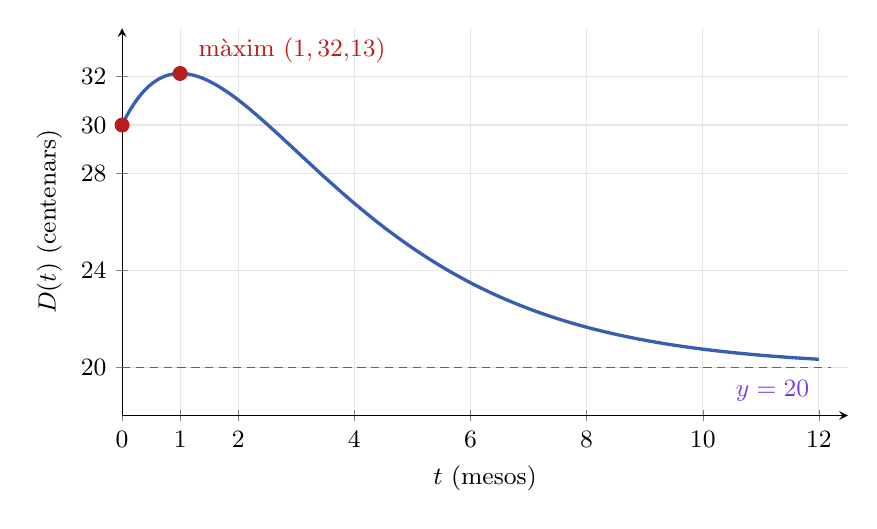
\begin{tikzpicture}
\begin{axis}[
  width=10.8cm,height=6.5cm,axis lines=left,
  xmin=0,xmax=12.5,ymin=18,ymax=34,
  xlabel={$t$ (mesos)},ylabel={$D(t)$ (centenars)},
  xtick={0,1,2,4,6,8,10,12},ytick={20,24,28,30,32},
  grid=major,grid style={black!10},tick label style={font=\small},label style={font=\small},clip=false]
  \addplot[corba,very thick,domain=0:12,samples=180]{20+10*(x+1)*exp(-x/2)};
  \addplot[asimptota,densely dashed,domain=0:12.2]{20};
  \addplot[only marks,mark=*,mark size=2.5pt,punt] coordinates {(0,30) (1,32.1306)};
  \node[anchor=south west,font=\small,text=punt] at (axis cs:1.15,32.15) {màxim $(1,32{,}13)$};
  \node[anchor=north east,font=\small,text=asimptota] at (axis cs:12,19.85) {$y=20$};
\end{axis}
\end{tikzpicture}
\end{document}
